\documentclass[12pt]{article}

\usepackage{algorithm2e}
\usepackage{amsmath}
\usepackage{cite}
\usepackage{fancyref}
\usepackage{float}
\usepackage[margin=1in]{geometry}
\usepackage{graphicx}
\usepackage{hyperref}
\usepackage{setspace}
\usepackage[nottoc,numbib]{tocbibind}

\title{Graph-based Semi-Supervised Learning for Text Categorization through Supervised Random Walks}
\author{
    Tom Shen \\
    \href{mailto:zhixians@andrew.cmu.edu}{zhixians@andrew.cmu.edu}
    \and
    William W. Cohen \\
    \href{mailto:wcohen@cs.cmu.edu}{wcohen@cs.cmu.edu}
}
\date{\today}

\begin{document}
\pagenumbering{roman}


\maketitle
\pagebreak

\singlespacing
\tableofcontents
\pagebreak

\doublespacing
\pagenumbering{arabic}

\begin{abstract}
Recently, many effective graph-based algorithms for semi-supervised learning have been developed.
These algorithms can often be applied to text classification tasks, since a similarity graph can be easily constructed from a set of text documents.
We introduce a graph-based semi-supervised learning algorithm based an algorithm used in ProPPR, a first-order probabilistic language for logical inference.
ProPPR answers queries by converting them to graphs and running an algorithm based on supervised random walks.
This algorithm was chosen for efficiency purposes and for suitability to the problem.
In this paper, we will show that this algorithm is also an effective algorithm for graph-based semi-supervised learning on its own, especially for text classification.
We compare it to two existing state-of-the-art algorithms, modified adsorption and Gaussian random fields, and show that it outperforms them on text classification tasks.
We will also show that the algorithm has comparable efficiency, and is easily parallelizable.
\end{abstract}
\pagebreak


\section{Introduction}

\subsection{Semi-Supervised Learning}
One of the core tasks in machine learning is \textit{supervised learning}.
Given labeled training data, a function that maps instances to labels is learned.
For many problems, very little labeled training data is available, since such data must often be labeled by humans.
However, a large amount of unlabeled data is often available.
\textit{Semi-supervised learning} (SSL) is a class of tasks and techniques where both a small amount of labeled training data and a large amount of unlabeled training data are available.
Commonly, rather than learning a function that maps arbitrary instances to labels, we instead want to find the labels for the unlabeled data. This is often called \textit{label propagation}.
A natural representation of SSL data is a graph constructed based on similarity between instances.
Common graph representations are bipartite graphs where documents are connected to their features, and $k$-nearest neighbor graphs, where documents are connected to other documents based on similarity.

\subsection{Text Classification}
A common problem in machine learning is \textit{text classification}.
Given a text document, we want to assign it to one or more categories.
Often, we are given a large set of documents and class labels for a small subset of them (called \textit{seed} documents), and we want to develop an algorithm that can assign class labels to all the documents.
This is a natural application of semi-supervised learning.

\subsection{Motivation}
Recently, a first-order probabilistic language for logical inference called ProPPR has been developed. \cite{wang2013programming}
It converts queries to graphs, and uses a graph-based semi-supervised learning method called \textit{supervised random walks} (SRW) to answer the queries.
We are interested in seeing how this method compares to state-of-the-art graph-based semi-supervised learning methods, such as Gaussian random fields\cite{zhu2003combining} and modified adsorption \cite{talukdar2009new,talukdar2010experiments}.

\subsection{Roadmap}
We start by discussing the background of ProPPR and SRW.
We also discuss the graph-based SSL methods we will be comparing ProPPR to, Gaussian random fields and modified adsorption.
We then review the datasets we will be using: 20 Newsgroups, WebKB, and Freebase.
We then explain the experimental setup we will be using to compare the algorithms.
Finally, we present the results of our experiments and analysis of the performance of the algorithms.

Overall, ProPPR's graph-based SSL method, SRW, performs better than existing methods on text classification tasks, and comparatively on other graph-based SSL tasks.
Additionally, it parallelizes fairly well.
Thus, SRW is an effective graph-based SSL method that should be considered for tasks beyond ProPPR.

\section{Background}
% problems suited to label propagation
% necessary properties of graphs, e.g. being \textit{homophilous}

\subsection{Personalized PageRank}
\textit{PageRank} \cite{page1999pagerank} is an algorithm developed to rank search engine results.
It is based on random walks on a graph with nodes representing web pages and edges representing links between pages, with a chance in each iteration of restarting on a random web page.

\textit{Personalized PageRank} (PPR) \cite{haveliwala2003analytical} is an extension of PageRank.
There is allowed to be biases towards specific nodes in the graph.
During an iteration of a random walk, jumps to nodes in the graph occur based on ``preference,'' which is represented with a normalized distribution of weights on the nodes in the graph.
Note that personalized PageRank can act as a distance metric in the graph, since nodes are more likely to jump to nodes with higher weights.

\subsection{ProPPR}
\textit{Programming with personalized PageRank} (ProPPR) \cite{wang2013programming} is a first-order probabilistic language for logical inference.
Traditionally, queries are answered through \textit{grounding}, by mapping them to propositional representations and then performing inference.
This is computationally expensive, since a large database of facts can lead to a large grounding.
ProPPR instead approximates ``local'' grounding by grounding every query with a small, labeled graph independent of database size.
Inference is then performed through PPR over a directed graph with feature-vector edges.

ProPPR uses an implementation of \textit{supervised random walks} (SRW), \cite{backstrom2011supervised} which were first developed as a method to predict links between nodes in a social network graph.
Given a graph with feature-vector annotated edges, a PPR process is performed.
This procedure is based on minimizing pairwise ranking loss.
In ProPPR, this pairwise ranking loss is decomposed into a positive-negative log loss function.
This function is then optimized with \textit{stochastic gradient descent} (SGD) rather than the quasi-Newton methods used by Backstrom and Leskovec.
SGD was chosen for speed and easy parallelization.

We are interested in seeing if ProPPR's backend (SRW) can be used on its own for label propagation.
In particular, we want to see how it compares to state-of-the-art label propagation methods, such as the ones listed below.

\subsection{Gaussian random fields}
\textit{Gaussian random fields} (GRF) \cite{zhu2003combining} is one of the earliest label propagation methods.
It ``prefers'' smooth labelings since the score of the label for a node is the weighted average of the scores for that label of the node's neighbors.
Additionally, label assignments where two nodes connected by a highly weighted edge but are assigned different labels are penalized.

\subsection{Modified adsorption}
\textit{Modified adsorption} (MAD) \cite{talukdar2009new,talukdar2010experiments} is a method based on {\it adsorption}. \cite{baluja2008video}
Adsorption is an algorithm that involves a random walk over a graph where, at each vertex $v$, we have probability
\begin{itemize}
\item $p_v^{inj}$ of stopping and returning (injecting) a predefined vector $Y_v$,
\item $p_v^{cont}$ of continuing the walk to a neighbor of $v$, randomly chosen with probabilities based on edge weights, and
\item $p_v^{abnd}$ of abandoning the walk and returning a zero vector.
\end{itemize}
MAD is an algorithm that retains most of the properties of the adsorption algorithm, but with a well-defined objective function to minimize.

\section{Prior Work}
Wang, Mazaitis, and Cohen \cite{wang2013programming} showed that the ProPPR system as a whole can be used to perform label propagation.
They demonstrated that it had comparable performance as the voted perceptron and contrastive divergence algorithms.

Lin and Cohen \cite{lin2010semi} compared MultiRankWalk, a random-walk based SSL algorithm, to weighted-vote relational neighbor classifiers and Gaussian random fields.
They showed that MultiRankWalk outperformed the other algorithms on a number of benchmark network datasets, with very little labeled data.

Talukdar and Pereira \cite{talukdar2010experiments} compared the graph-based SSL algorithms modified adsorption, adsorption, and Gaussian random fields on a number of graph datasets, including Freebase 1 and Freebase 2.
They demonstrated that modified adsorption outperforms other state-of-the-art graph algorithms.


\section{Experimental Results}
We are interested in seeing how ProPPR's implementation of supervised random walks compares to other graph-based semi-supervised learning algorithms.

\subsection{Algorithms}
We compare three different algorithms:
\begin{enumerate}
\item Gaussian random fields (GRF)
\item Modified adsorption (MAD)
\item ProPPR's supervised random walks (SRW)
\end{enumerate}

We use implementations of GRF (called LP-ZGL) and MAD from the Junto Label Propagation Toolkit \footnote{\url{https://github.com/parthatalukdar/junto}}.

We base our implementation of SRW on the Java implementation of ProPPR \footnote{\url{https://github.com/TeamCohen/ProPPR}}. Since the graphs we use are all undirected with a single weight on each edge, we first convert them to directed graphs with a feature vector on each edge.

We generate a new graph for each class by adding a special start node to the instance graph, and adding an edge from the start node to the node for each seed instance for that class.
Thus, a random walk in the graph will start with the seed instances, and then proceed to their neighbors, which are the instances most similar to them.

After running ProPPR's SRW algorithm on each of these graphs, each node in each graph will have an associated weight.
The weight of a node in a graph represents how highly associated that node is with the class corresponding to that graph.
Thus, we can form a ranked list of class labels for each node based on its weights in the class graphs.

Psuedocode for the algorithm can be seen in Algorithm~\ref{fig:srw}.

\begin{algorithm}
  \KwIn{Undirected, weighted graph $G = (V,E)$, mapping of seed nodes to labels $S$, list of labels $L$}
  \KwOut{Mapping of nodes to ranked list of labels $R$}
  Let $V' = V$, $E = []$\;
  Create directed, feature-vector weighted graph $G' = (V',E')$\;
  Add start node $s$ to $V'$\;
  \For{$(u,v,w) \in E$}{
    Add $(u,v)$ with feature vector $[w,0]$ to $E'$\;
    Add $(v,u)$ with feature vector $[w,0]$ to $E'$\;
  }
  Let $R = \{ v \mapsto [] \mid v \in V \}$\;
  \For{$l \in L$}{
    Let $G''=(V'',E'')$ be a copy of $G'$\;
    \For{$(v \mapsto l') \in S$} {
      \If{$l = l'$}{
        Add $(s,v)$ with feature vector $[0,1]$ to $E''$\;
      }
    }
    Run SRW on $G''$, and let $M$ be the output\;
    \For{$v \in V$}{
      Append $(M[v], l)$ to $R[v]$\;
    }
  }
  \For{$v \in V$}{
    Sort in descending order $R[v]$\;
  }
  \caption{Psuedocode for SRW. Note that we can easily parallelize across the classes.\label{fig:srw}}
\end{algorithm}

\subsection{Datasets}
We use four datasets suitable for graph-based semi-supervised learning: Freebase 1, Freebase 2, 20 Newsgroups, and WebKB.
Freebase 1 and Freebase 2 are derived from a \textit{knowledge base}, which is a graph of topics their relations.
They are not text classification datasets, but since they have been used to measure performance of other graph-based SSL algorithms \cite{talukdar2010experiments}, we use them to measure performance as well.

\begin{table}[h]
\centering
\begin{tabular}{|l|l|l|l|}
\hline
\textbf{Name} & \textbf{Nodes} & \textbf{Edges} & \textbf{Classes} \\ \hline
Freebase 1    & 32970             & 957076         & 46               \\ \hline
Freebase 2    & 301638            & 2310002        & 384              \\ \hline
20NG & 79962             & 2435219        & 20               \\ \hline
WebKB & 11969             & 324254        & 4               \\ \hline
\end{tabular}
\caption{Statistics for the dataset graphs}
\label{dataset-stats}
\end{table}

Freebase \cite{freebase:datadumps,talukdar2010experiments} is a collaborative knowledge base that uses information from both open data sets and user contributions.
\textbf{Freebase 1} is constructed from a small subset of relations from that knowledge base, covering topics from the domains: \textit{astronomy, automotive, biology, book, business, chemistry, comic books, computer, film, food, geography, location, people, religion, spaceflight, tennis, travel, \textnormal{and} wine}.
\textbf{Freebase 2} is a larger subset of relations constructed in the same fashion and covering the same domains.

\textbf{20 Newsgroups} (20NG) \cite{Lang95} is a collection of 18,774 newsgroup documents (emails).
There are 61,188 words, and 20 different classes, one for each newsgroup: \textit{comp.graphics, comp.os.ms-windows.misc, comp.sys.ibm.pc.hardware, comp.sys.mac.hardware, comp.windows.x, rec.autos, rec.motorcycles, rec.sport.baseball, rec.sport.hockey, sci.crypt, sci.electronics, sci.med, sci.space, misc.forsale, talk.politics.misc, talk.politics.guns, talk.politics.mideast, talk.religion.misc, alt.atheism, \textnormal{and} soc.religion.christian}.
A subset of the graph for 20 Newsgroups can be seen in Figure~\ref{fig:20ng}. Emails are connected to words that they contain, with edges weighted by word count.

\begin{figure}[H]
    \centering
    \includegraphics[width=0.7\textwidth]{figures/20ng.pdf}
    \caption{Subset of 20 Newsgroups graph\label{fig:20ng}}
\end{figure}

\textbf{WebKB} \cite{cachopo2007improving} is a set of 4199 web pages collected by the World Wide Knowledge Base project, from computer science departments of four universities (Cornell, Texas, Washington, Wisconsin) in 1997.
We are using a subset of the pages with four classes: \textit{student, faculty, course, \textnormal{and} project}.

All datasets are in the form of undirected graphs with weighted edges.

\subsection{Environment}
Unless otherwise noted, all implementations are given access to 8 GB of memory and are run single-threaded.

\subsection{Seed selection}
We choose seeds in two different ways: entirely randomly, and based on highest out-degree.
Randomly choosing seeds is reasonable, since, for real datasets, often arbitrary instances are labeled.
Nodes with highest out-degree are those that are ``influential,'' since propagation through those nodes has the potential to affect the greatest number of other nodes.
And often, for real datasets, the most influential instances will be those that we have the labels for.

We choose $1\%$, $5\%$ and $10\%$ of the instances as seeds. These represent three typical small proportions of labeled data compared to unlabeled data.

\subsection{Evaluation}
We evaluate the performance based on two metrics:

\textit{Mean reciprocal rank} (MRR) is a statistical measure that represents how highly the correct classes are ranked for each node's ranked list of class labels:
$$\textnormal{MRR} = \frac{1}{|Q|} \sum_{v \in Q} \frac{1}{\textnormal{rank}_v}$$
where $Q$ is the set of test nodes, and $\textnormal{rank}_v$ is the rank of the correct class label in the list of classes assigned to the node $v$.

\textit{$F_1$ score} is a measure of accuracy based on the precision $p$ and recall $r$:
$$F_1 = 2 \cdot \frac{p \cdot r}{p + r}$$

A node is considered positive if its highest ranked class is the correct class.

\subsection{Parallelism}
To test parallel performance, we run SRW on the two largest datasets, Freebase 2 and 20 Newsgroups, with varying numbers of threads.
Parallelism is achieved by performing the run of SRW on each label's graph in a separate thread.

\subsection{Results}
SRW performs substantially better than GRF and MAD on the two text classification datasets, 20NG and WebKB, for all proportions of seeds and methods of seed selection, except on $MRR$ for random seeds.
SRW has a better $F_1$ score but worse $MRR$ on the other two graph datasets, $Freebase 1$ and $Freebase 2$.
Thus, in all cases, SRW has comparable performance, and it outperforms the other two algorithms on the text classification datasets.

\begin{figure}[p]
    \subsection{Freebase 1}
    \centering
    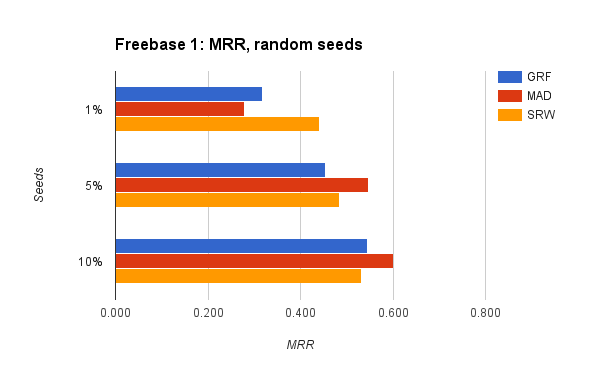
\includegraphics[width=0.49\textwidth]{figures/freebase1-mrr-random}
    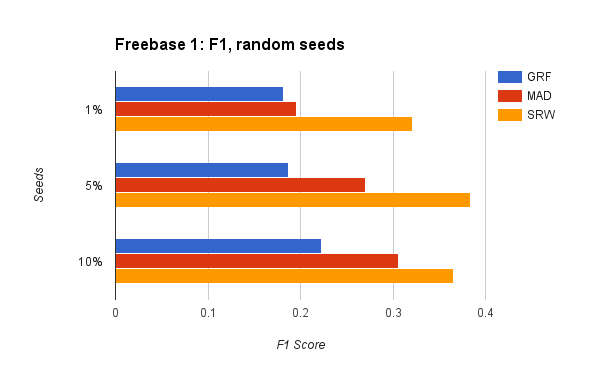
\includegraphics[width=0.49\textwidth]{figures/freebase1-f1-random}
    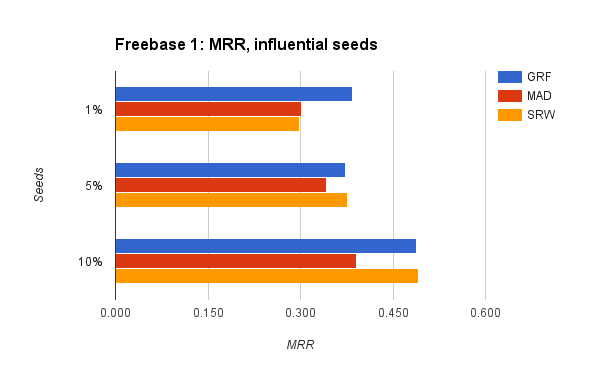
\includegraphics[width=0.49\textwidth]{figures/freebase1-mrr-top}
    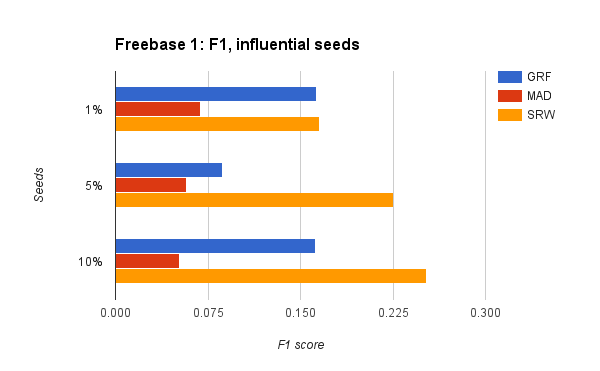
\includegraphics[width=0.49\textwidth]{figures/freebase1-f1-top}
    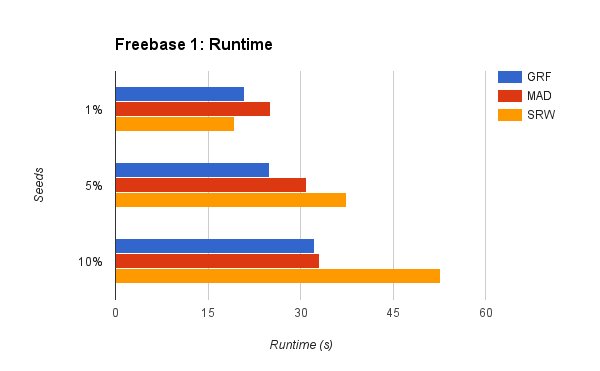
\includegraphics[width=0.8\textwidth]{figures/freebase1-runtime}
    \caption{Freebase 1}
\end{figure}

\begin{figure}[p]
    \subsection{Freebase 2}
    \centering
    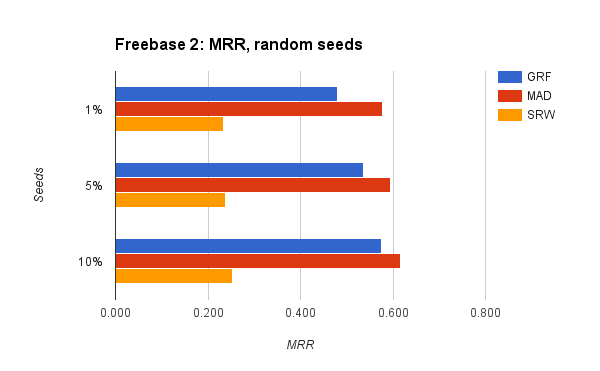
\includegraphics[width=0.49\textwidth]{figures/freebase2-mrr-random}
    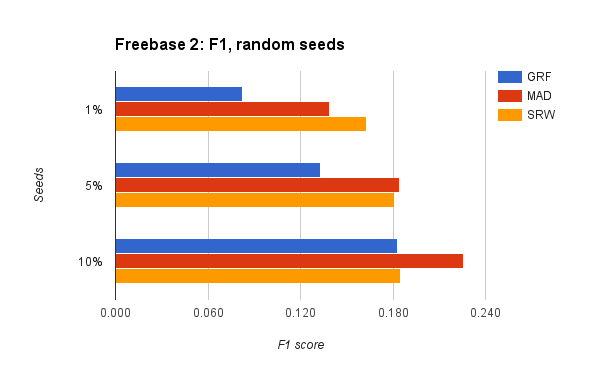
\includegraphics[width=0.49\textwidth]{figures/freebase2-f1-random}
    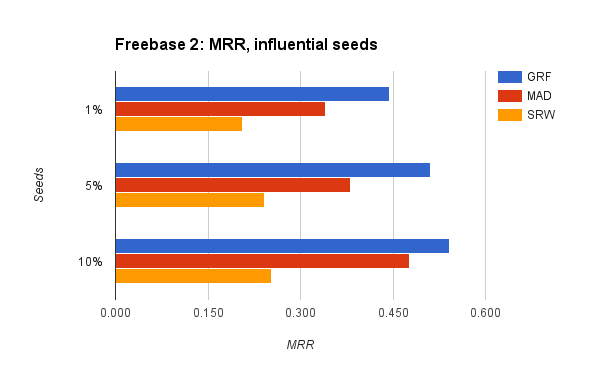
\includegraphics[width=0.49\textwidth]{figures/freebase2-mrr-top}
    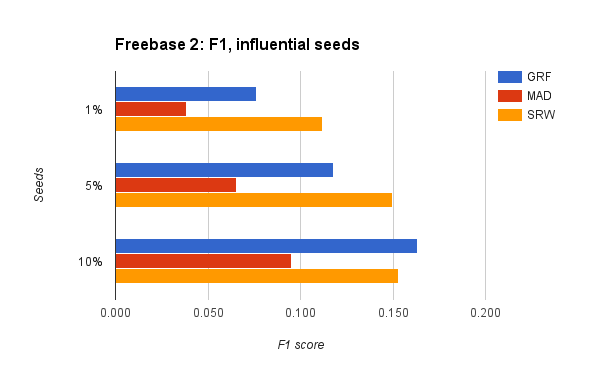
\includegraphics[width=0.49\textwidth]{figures/freebase2-f1-top}
    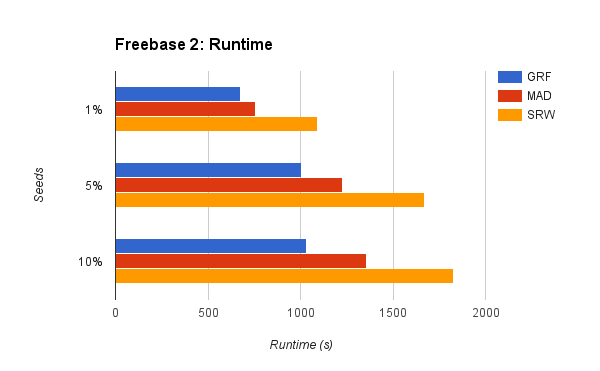
\includegraphics[width=0.8\textwidth]{figures/freebase2-runtime}
    \caption{Freebase 2}
\end{figure}

\begin{figure}[p]
    \subsection{20 Newsgroups}
    \centering
    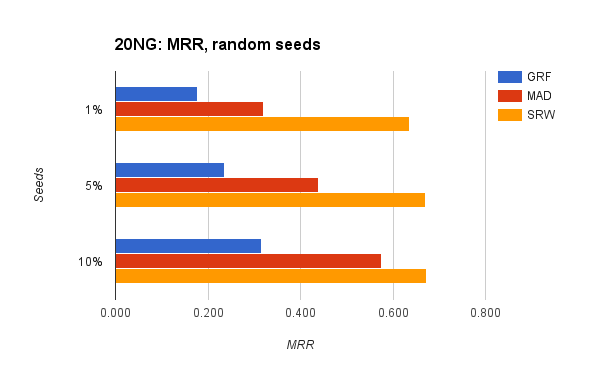
\includegraphics[width=0.49\textwidth]{figures/20ng-mrr-random}
    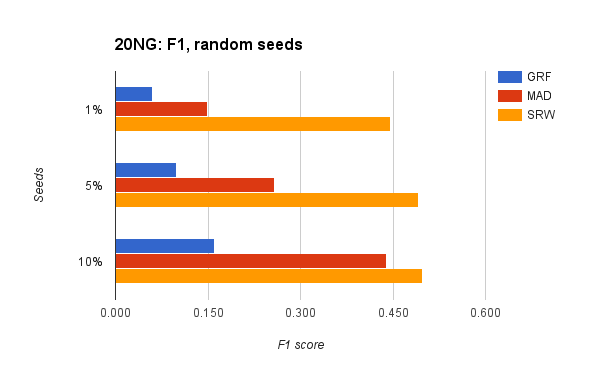
\includegraphics[width=0.49\textwidth]{figures/20ng-f1-random}
    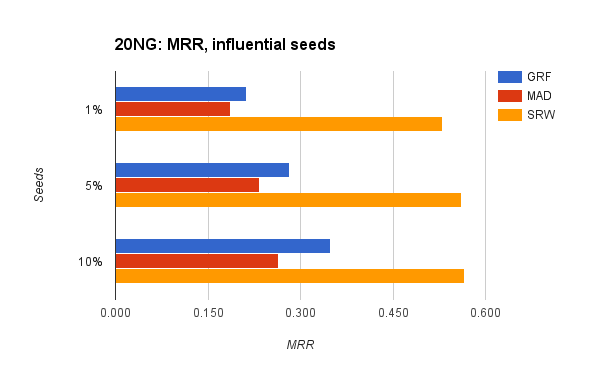
\includegraphics[width=0.49\textwidth]{figures/20ng-mrr-top}
    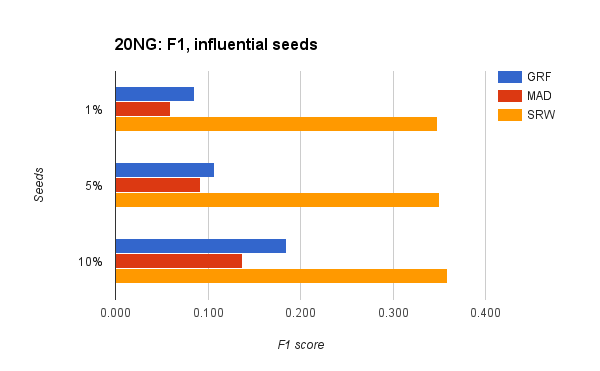
\includegraphics[width=0.49\textwidth]{figures/20ng-f1-top}
    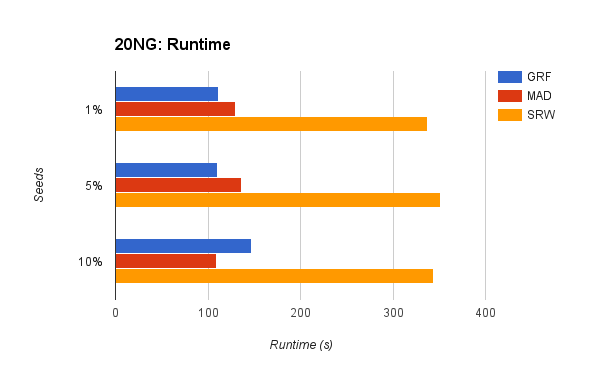
\includegraphics[width=0.8\textwidth]{figures/20ng-runtime}
    \caption{20NG}
\end{figure}

\begin{figure}[p]
    \subsection{WebKB}
    \centering
    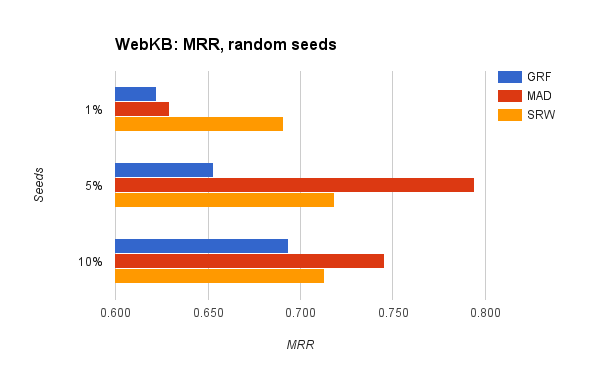
\includegraphics[width=0.49\textwidth]{figures/webkb-mrr-random}
    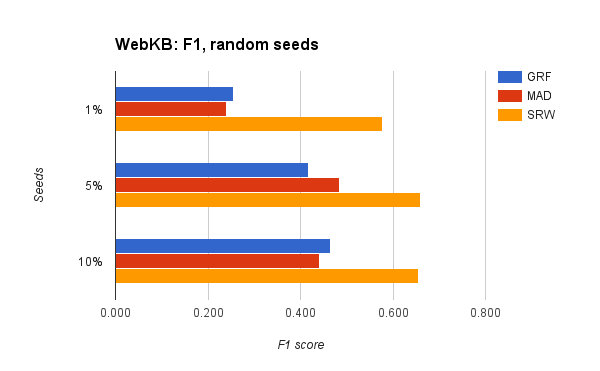
\includegraphics[width=0.49\textwidth]{figures/webkb-f1-random}
    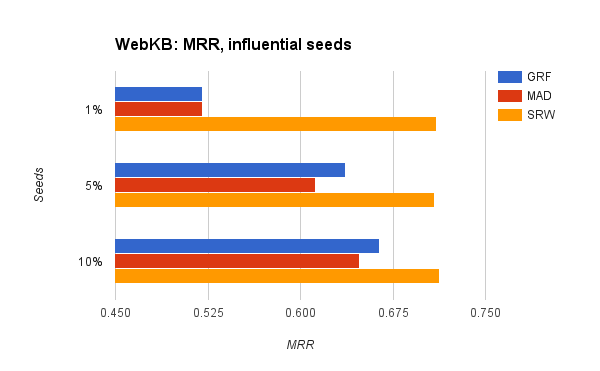
\includegraphics[width=0.49\textwidth]{figures/webkb-mrr-top}
    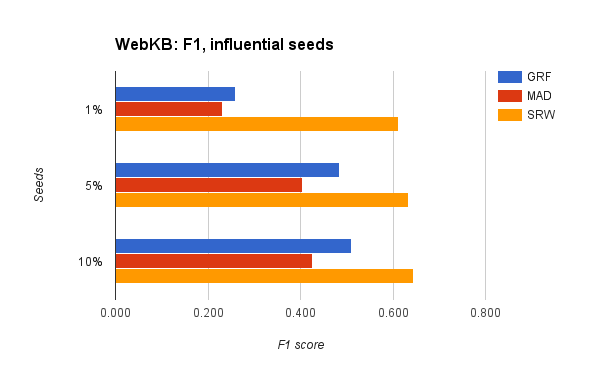
\includegraphics[width=0.49\textwidth]{figures/webkb-f1-top}
    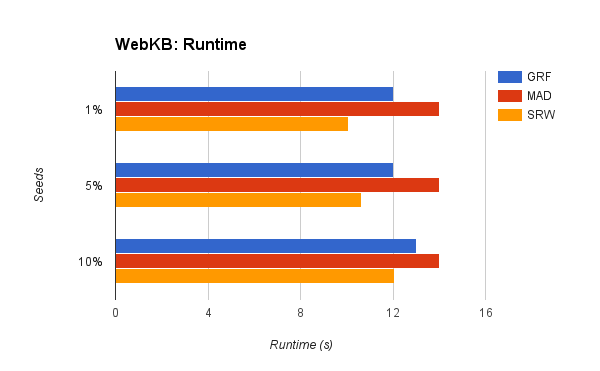
\includegraphics[width=0.8\textwidth]{figures/webkb-runtime}
    \caption{WebKB}
\end{figure}

\pagebreak


\section{Analysis}

\subsection{Runtime}
Overall, the runtime of SRW is comparable to that of MAD and GRF.
Though it is slower on 20NG and Freebase 2, the difference in runtime is a constant factor that does not appear to depend on number of instances.

\begin{figure}[h]
    \centering
    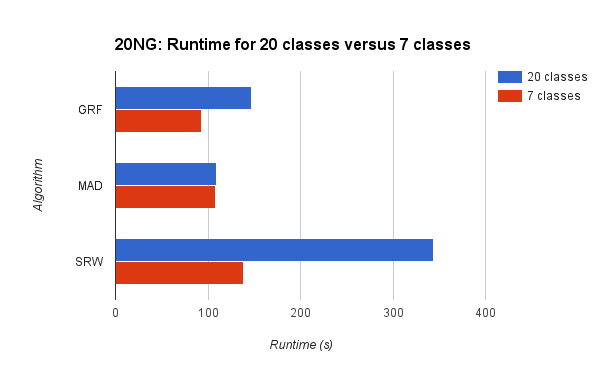
\includegraphics[width=0.8\textwidth]{figures/20ng-classes}
    \caption{20NG: 20 classes versus 7 classes\label{fig:classes}}
\end{figure}
Reducing the number of classes without changing then number of instances does affect the runtime of SRW significantly.
To demonstrate this, we generated a new graph by combining the 20 classes in 20NG into seven, based on the category each mailing list falls under: \textit{comp.*, rec.*, sci.*, misc.*, talk.*, alt.*, \textnormal{and} soc.*}.
In this way, class labels still make sense, since they simply become more general, and the number of instances does not change.
As seen in Figure~\ref{fig:classes}, reducing the number of classes leads to a proportional decrease in runtime for SRW, but not for GRF or MAD.
This makes sense, since the algorithm must generate a graph and run a supervised random walk for each class in the dataset.

\subsection{Parallelism}

\begin{figure}[H]
    \centering
    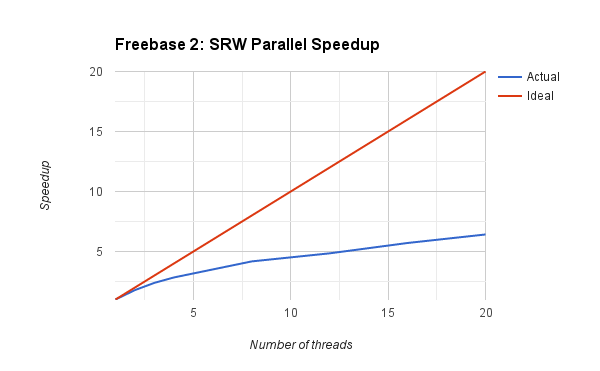
\includegraphics[width=0.8\textwidth]{figures/freebase2-speedup}
    \includegraphics[width=0.8\textwidth]{figures/20NG-speedup}
    \caption{SRW speedup from using threads on 20NG and Freebase 2\label{fig:speedup}}
\end{figure}
SRW benefits from parallelization up to 4 threads, and then speedup falls off significantly.
This can be attributed to substantial communication costs.
A copy of the instance graph must be made for each thread, and threads must send the weights for all the nodes in the graph after completion.
Additionally, generating the ranked list of class labels for each node is inherently highly sequential.
Still, reasonable speedup can be achieved through use of a small number of threads.

\section{Conclusion}
Overall, SRW has been shown to be not just an effective component of the ProPPR solver system, but also as a standalone graph-based SSL method for text classification.
It has better performance than existing state-of-the-art graph-based SSL methods on text classification problems, and comparable performance on more general graph-based datasets.
Additionally, its speed is comparable or slightly slower, and it can be easily parallelized for significant speedup.


\section{Future Work}
The runtime of supervised random walks is directly proportional to number of classes, since it runs the algorithm on a graph generated for each class.
Since the same is not true for Gaussian random fields and modified adsorption, we could investigate adapting parts of those algorithms to improve performance of SRW on datasets with many classes.
Additionally, speedup from parallelization falls off at a certain point, so we could investigate reducing communication costs and sequential work to improve parallel performance.


\bibliographystyle{siam}
\bibliography{references}{}


\end{document}
